% !TEX encoding = UTF-8 Unicode
% !TEX TS-program = pdflatex
% !TEX root = ../Tesi.tex


%************************************************
\myChapter{Il problema elettromagnetico}
%************************************************
\label{cap:maxwell}

\section{Equazioni di Maxwell}

La simulazione numerica elettromagnetica implica la risoluzione delle \textit{equazioni di Maxwell}, qui richiamate in forma puntuale:

\begin{equation}
	\label{eq:2max1}
	\rot\left(\T{e}\right)=-\partial_t \T{b},
\end{equation}

\begin{equation}
	\label{eq:2max2}
	\dive\left(\T{d}\right)=\rho,
\end{equation}

\begin{equation}
	\label{eq:2max3}
	\rot\left(\T{h}\right)=\T{j}+\partial_t \T{d},
\end{equation}

\begin{equation}
	\label{eq:2max4}
	\dive\left(\T{b}\right)=0,
\end{equation}
dove $\T{e} \; \left( \frac{\text{V}}{\text{m}} \right)$ e $\T{h} \; \left( \frac{\text{A}}{\text{m}} \right)$ sono rispettivamente le intensità di campo elettrico e magnetico, mentre $\T{d} \; \left( \frac{\text{C}}{\text{m}^2} \right)$ e $\T{b} \; \left( \frac{\text{Wb}}{\text{m}^2} \right)$ sono i vettori induzione elettrica e magnetica. 
\begin{SCfigure}[1.8][htp]
\caption{Superficie di riferimento per il teorema di Stokes, utilizzato nelle Eq. \eqref{eq:2faraday} e \eqref{eq:2ampere2}}
\label{fig:2.1}
\tdplotsetmaincoords{55}{45}
\begin{tikzpicture}
	[scale=2,
		tdplot_main_coords,
		curve/.style={draw = black,fill = black!10!white, opacity = .7}]
\def\R{.8} % sphere radius
\coordinate (O) at (0,0,0);
\coordinate (A) at (0,0,1);
\coordinate (B) at (0,\R,0);
\coordinate (C) at (0,0,-1);
%draw the circle in the main frame
\tdplotdrawarc[curve]{(O)}{\R}{0}{360}{}{}
\draw[->] {(O) -- (A)};
\draw (A) node[right] {$\T{n}$}; %label
\draw (\R*.4,0,0) node[right] {$S$}; %label
\draw (0, \R, 0) node[right] {$\partial S$}; %label
\end{tikzpicture}
\end{SCfigure}

L'equazione \eqref{eq:2max1} ha come forma integrale la \textit{legge di Faraday} (o \textit{legge dell'induzione elettromagnetica})che lega la circuitazione dell'intensità di campo elettrico lungo una linea chiusa alla variazione di flusso di induzione magnetica attraverso la superficie racchiusa:
\begin{equation}
\label{eq:2faraday}
\int_{\partial S} \T{e}\cdot d\T{l} = -\partial_t \int_S \T{b} \cdot d\T{s}.
\end{equation}

\begin{SCfigure}[2.5][htp]
\caption{Volume di riferimento per il teorema di Gauss, utilizzato in Eq. \eqref{eq:2gauss}}
\label{fig:2.2}
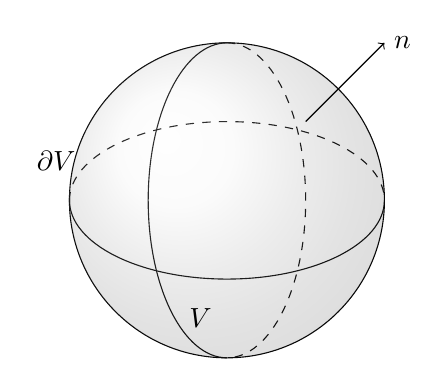
\begin{tikzpicture}
    \draw (-2,0) arc (180:360:2cm and 1cm);
    \draw[dashed] (-2,0) arc (180:0:2cm and 1cm);
    \draw (0,2) arc (90:270:1cm and 2cm);
    \draw[dashed] (0,2) arc (90:-90:1cm and 2cm);
    \draw (0,0) circle (2cm);
    \shade[ball color=black!10!white,opacity=0.20] (0,0) circle (2cm);
    \draw[->] {(1,1) -- (2,2)};
    \draw (2,2) node[right] {$\T{n}$}; %label
    \draw (-1.8,0.5) node[left] {$\partial V$}; %label
    \draw (-.6,-1.5) node[right] {$V$}; %label
\end{tikzpicture}\end{SCfigure}

L'equazione \eqref{eq:2max2} è il \textit{teorema di Gauss} applicato al campo elettrico:
\begin{equation}
\label{eq:2gauss}
\int_{\partial V} \T{d} \cdot d\T{s}= Q_{enc} = \int_V \rho dv,
\end{equation}
dove $Q_{enc}$ è la carica totale racchiusa nel volume $V$ circondato dalla superficie $\partial V$, e $\rho$ è la densità di carica per unità di volume.
\\
L'equazione \eqref{eq:2max3} è il risultato della modifica apportata da Maxwell alla \textit{legge di  Ampère}, in origine:
\[
\int_{\partial S} \T{h} \cdot d\T{l} = i_{enc} = \int_S \T{j} \cdot d\T{s},
\]
dove $i_{enc}$ è la corrente totale che attraversa la superficie $S$, e $\T{j}$ è la densità di corrente per unità di superficie (\textit{corrente volumetrica}).

Il termine $\partial_t \T{d}$ (che Maxwell ha nominato \textit{corrente di spostamento}) porta alla simmetria delle equazioni e alla forma integrale:
\begin{equation}
\label{eq:2ampere2}
\int_{\partial S} \T{h} \cdot d\T{l} = \int_S \left( \T{j} + \partial_t \T{d} \right) \cdot d\T{s}.
\end{equation}

Infine l'equazione \eqref{eq:2max4} rappresenta la solenoidalità dell'induzione magnetica $\T{b}$:
\begin{equation}
\label{eq:2solen}
\int_{\partial V} \T{b} \cdot d\T{s} = 0.
\end{equation}

Si noti che applicando la divergenza ad entrambi i termini dell'equazione \eqref{eq:2max3} si può ottenere il legame tra cariche e correnti elettriche. Questo legame è pertanto implicito nella definizione del problema:
\begin{align}
\label{eq:2corr1}
\dive \left[ \rot\left(\T{h}\right) \right] &= \dive \left(\T{j}+\partial_t \T{d} \right) \nonumber\\
0&=\dive \left(\T{j}\right) + \partial_t \dive \left(\T{d}\right) \nonumber\\
0&=\dive \left(\T{j}\right) + \partial_t\rho\nonumber\\
\partial_t \rho &= - \dive \left(\T{j}\right).
\end{align}

\section{Legami costitutivi}

Per definire le interazioni fra le diverse equazioni occorre indagare i legami tra le intensità di campo e le rispettive induzioni; tali relazioni dipendono dalla natura del dominio in cui vengono applicate le equazioni. 

Nel vuoto si hanno le ben note relazioni:
\begin{equation}
\label{eq:2cost}
\left\{
\begin{aligned}
\T{d} &= \varepsilon_0 \T{e}\\
\T{b} &= \mu_0 \T{h}
\end{aligned}
\qquad\text{con}\qquad
\begin{aligned}
\varepsilon_0&=8{,}854\,187\,817\,62\cdot 10^{-12} &\frac{\text{F}}{\text{m}}\\
\mu_0&= 1{,}256\,637\,061\,44\cdot10^{-6} &\frac{\text{H}}{\text{m}}
\end{aligned}
\right.
\end{equation}

A queste si aggiunga la relazione tra il campo elettrico all'interno di un materiale e la corrente generata all'interno dello stesso (\textit{conduction current}):
\begin{equation}
\label{eq:2conduction_current}
\T{j}=\T{j_c}+\T{j_i}, \qquad \text{con}\qquad \T{j_c}=\sigma \T{e}
\end{equation}
dove $\T{j_i}$ è la \textit{corrente impressa} e $\sigma$ è la conduttività del materiale. 

Nel vuoto si ha:
\[
\sigma=0
\]
Nei prossimi paragrafi verrà brevemente giustificata la natura delle leggi costitutive in seguito utilizzate.


\subsection{Campi elettrici nella materia}
\label{subsec:elecmateria}
La risposta di un materiale alle sollecitazioni del campo elettrico varia in base alla natura del materiale stesso. 

Identifichiamo due grandi classi di materiali: \textit{isolanti} (o \textit{dielettrici}) e \textit{conduttori}. In un materiale isolante ciascun elettrone è legato ad uno specifico atomo, mentre in un conduttore gli elettroni (o gli ioni per i conduttori liquidi) sono liberi di spostarsi fra i diversi nuclei.
\begin{itemize}
\item[\textit{Isolanti}]
Quando un materiale dielettrico viene sottoposto ad un campo elettrico ciascun atomo (neutro) è sottoposto ad una forza totale nulla; tuttavia nuclei ed elettroni sono sottoposti a forze uguali ed opposte, a causa della loro carica non nulla tali forze tendono quindi ad allontanare nucleo ed elettroni. Eccezion fatta per i casi in cui tale forza è così alta da separarli completamente (ionizzando l'atomo) viene raggiunta una nuova configurazione di equilibrio tra le forze interne di attrazione fra nucleo ed elettroni e le forze indotte dal campo elettrico esterno. 

In questa configurazione l'atomo è detto \textit{polarizzato} e possiede un momento di dipolo $\T{p_a}$  parallelo al campo elettrico e ad esso proporzionale tramite la \textit{polarizzabilità} $\alpha$:
\begin{equation}
\label{eq:2polar1}
\T{p} = \alpha \left(\T{e}\right)\cdot \T{e}.
\end{equation}

Considerando intere molecole anziché singoli atomi la polarizzazione può seguire direzioni preferenziali e non essere pertanto parallela al campo elettrico.
Più in generale si ha quindi:
\begin{equation}
\label{eq:2polar2}
\T{p_m} = \TT{\alpha} \left( \T{e} \right) \cdot\T{e},
\end{equation}
dove $\TT{\alpha}$ è un tensore del II ordine (tensore di polarizzabilità).
In questa configurazione il campo elettrico esterno esercita una coppia sulle molecole che tende ad allineare i dipoli con il campo stesso:
\begin{equation}
\label{eq:2polar3}
\T{C_p}=\T{p_m} \times \T{e}.
\end{equation}

Il campo elettrico esercita quindi due azioni sulle molecole: distorsione e rotazione. Entrambe portano allo stesso risultato: il dielettrico presenta un numero di dipoli allineati in una direzione preferenziale.

Definiamo quindi per un materiale dielettrico il vettore $\T{p}$ (\textit{polarizzazione}) come la densità di momenti di dipolo. Questo campo è la sintesi dell'effetto che le cariche generate dal campo elettrico esterno esercitano sul campo elettrico stesso.
Le cariche sono esprimibili tramite il vettore di polarizzazione come:
\begin{equation}
\label{eq:2charges1}
\left\{
\begin{aligned}
\rho_{b} &= -\dive \left(\T{p}\right) \qquad &\text{in $V$}\\
\sigma_{b} &= \T{p}\cdot \T{n} \qquad &\text{in $S$}.
\end{aligned}
\right.
\end{equation}
 
Riscrivendo l'equazione \eqref{eq:2gauss} nel dominio del materiale, utilizzando la prima delle \eqref{eq:2cost} e aggiungendo le cariche dovute alla polarizzazione si ha:
\begin{align}
\label{eq:2polar3}
&\int_S \varepsilon_0\T{e} \cdot d\T{s}  = \int_V \left( \rho+\rho_{b}\right) dv\nonumber\\
&\int_S \varepsilon_0\T{e} \cdot d\T{s}  = \int_V \left[ \rho-\dive\left(\T{p}\right)\right] dv\nonumber\\
&\int_V \dive\left[\varepsilon_0\T{e} + \T{p} \right]\cdot dv  = \int_V \rho dv,\nonumber
\end{align}
da cui:
\begin{equation}
\label{eq:2polar4}
\T{d} = \varepsilon_0 \T{e} + \T{p}\left(\T{e}\right).
\end{equation}

Un caso comune è quello in cui la polarizzazione è proporzionale al campo elettrico:
\begin{equation}
\label{eq:2polar5}
\T{p} = \varepsilon_0 \TT{\chi_e} \T{e},
\end{equation}
dove  il tensore del II ordine $\TT{\chi_e}$ è detto \textit{suscettibilità elettrica}.

L'equazione \eqref{eq:2polar4} porta a:
\begin{equation}
\begin{split}
\label{eq:2polar6}
\T{d} &= \left[\varepsilon_0 \TT{I}+ \TT{\chi_e}\left(\T{e}\right)\right]\T{e} \\
      &= \TT{\varepsilon}\T{e}.
\end{split}
\end{equation}

Per materiali con proprietà dielettriche isotrope si può considerare il campo $\T{p}$ sempre parallelo a $\T{e}$. 

In questo caso si può scrivere:
\begin{equation}
\begin{split}
\label{eq:2costel}
\T{d} &= \left[\varepsilon_0+ \chi_e\left(\T{e}\right)\right]\T{e} \\
      &= \varepsilon\T{e}.
\end{split}
\end{equation}
\item[\textit{Conduttori}] La relazione \eqref{eq:2conduction_current} è applicabile a tutti i materiali, ma assume un ruolo non trascurabile solo se la conduttività del materiale è rilevante. Maggiore è $\sigma$ minore è il campo elettrico all'interno del materiale (in assenza di correnti impresse).
Al limite, identifichiamo come conduttore elettrico perfetto (\textit{Perfect Electric Conductor, PEC}) il materiale per cui:
\begin{equation}
\label{eq:2pec}
\sigma \rightarrow \infty,\qquad \T{e}\rightarrow 0.
\end{equation}
Questo modello è utile per rappresentare adeguatamente regioni metalliche che non costituiscono zone d'interesse per l'analisi; queste possono essere quindi escluse dal dominio di analisi e sostituite con adeguate condizioni al contorno. 
Nel caso in cui sia di primario interesse lo sviluppo dei campi elettromagnetici all'interno del conduttore (ad esempio nell'analisi di correnti parassite) il materiale deve essere adeguatamente modellato ed incluso nel dominio di analisi: 
\begin{align}
\label{eq:2pec2}
\T{d} &= \varepsilon\T{e},\\
\T{j} &= \T{j_i}+\sigma\T{e}.
\end{align}
Esistono tuttavia modelli semplificati adeguati all'analisi specifica di questa classe di problemi \citep{zaglmayr_high_2006}.
\end{itemize}
\subsection{Campi magnetici nella materia}
Proprietà analoghe possono essere mostrate anche per la controparte magnetica.

Gli elettroni appartenenti agli atomi di un materiale non magnetizzato, in quanto cariche in movimento dal periodo estremamente basso possono essere rappresentati come correnti stazionarie (lungo le loro orbite) di intensità:
\begin{equation}
\label{eq:2current1}
i=\frac{e}{T}=\frac{e v}{2 \pi R}.
\end{equation}

Si ricorda che una spira percorsa da corrente stazionaria è soggetta ad un momento meccanico:
\begin{equation}
\T{\tau}=\T{m}\times\T{b}, 
\end{equation}
\label{eq:2torque}
dove $\T{m}$ è detto \textit{momento di dipolo magnetico} ed è dato da
\begin{equation}
\label{eq:2mom}
\T{m}=i S \T{\hat{z}} = -\frac{1}{2}evR\T{\hat{z}}\quad \text{($S$ è la superficie racchiusa dall'orbita).}
\end{equation}
\begin{SCfigure}[2.4][htp]
\caption{Orbita di un elettrone attorno al nucleo e relativo momento di dipolo magnetico}
\label{fig:2.3}
\tdplotsetmaincoords{55}{45}
\begin{tikzpicture}
	[scale=2,
		tdplot_main_coords,
		curve/.style={draw = black,fill = black!10!white, opacity = .7},
		curve2/.style={black,->}]
\def\R{.8} % sphere radius
\coordinate (O) at (0,0,0);
\coordinate (A) at (0,0,1);
\coordinate (B) at (0,\R,0);
\coordinate (C) at (0,0,-1);
%draw the circle in the main frame
\draw[->] {(O) -- (C)};
\draw (C) node[right] {$\T{m}$}; %label
\tdplotdrawarc[curve]{(O)}{\R}{0}{360}{}{}
\tdplotdrawarc[curve2]{(O)}{\R*1.2}{320}{400}{}{}
\draw[->] {(O) -- (A)};
\draw[->] {(O) -- (B)};
\draw (A) node[right] {$\T{\hat{z}}$}; %label
\draw (B) node[right] {$-e$}; %label
\draw (\R*1.3,0,0) node[right] {$v$}; %label
\draw (0, \R/2, 0) node[right] {$R$}; %label
\end{tikzpicture}
\end{SCfigure}

La normale all'orbita dell'elettrone tende pertanto ad allinearsi con il campo magnetico.

In analogia con la polarizzazione, definiamo qui la \textit{magnetizzazione} $\T{m}\left(\T{h}\right)$ come la densità di momenti di dipolo magnetico.

Gli effetti dovuti alla magnetizzazione possono essere riassunti in una distribuzione di correnti equivalenti, volumetriche e superficiali:
\begin{equation}
\label{eq:2current2}
\left\{
\begin{aligned}
\T{j_{b}} &= \rot \left(\T{m}\right) \qquad &\text{in $V$}\\
\T{k_{b}} &= \T{m}\times \T{\hat{n}} \qquad &\text{in $S$}.
\end{aligned}
\right.
\end{equation}

Scriviamo ora il teorema di Ampère (Eq. \eqref{eq:2ampere2}) utilizzando il legame costitutivo \eqref{eq:2cost}:
\begin{align}
\label{eq:2current3}
&\oint_L \frac{1}{\mu_0}\T{b} \cdot d\T{l}  = \int_S \left( \T{j}+\T{j_{b}}+\partial_t\T{d}\right) d\T{s}\nonumber\\
&\oint_L \frac{1}{\mu_0}\T{b} \cdot d\T{l}  = \int_S \left( \T{j}+\rot\left(\T{m}\right)+\partial_t\T{d}\right) d\T{s}\nonumber\\
&\int_S \rot\left(\frac{1}{\mu_0}\T{b}-\T{m}\right) \cdot d\T{s}  = \int_S \left( \T{j}+\partial_t\T{d}\right) d\T{s},
\end{align}
che porta alla relazione costitutiva per il materiale magnetizzato:

\begin{equation}
\label{eq:2current4}
\T{b}=\mu_0\left(\T{h}+\T{m}\right).
\end{equation}

La natura di $\T{m}$ dipende fortemente dal tipo di materiale cui si fa riferimento. Si può assumere che in base al loro comportamento, i materiali di più comune interesse ricadano in una delle seguenti categorie \citep{furlani_permanent_2001}:
\begin{description}
\item[Paramagnetici]Gli atomi o le molecole di questi materiali hanno un momento netto, ma non vi è relazione fra le direzioni dei momenti adiacenti. Se sottoposti ad un campo magnetico i momenti tendono ad allinearvisi; l'allineamento è randomatico e dipende dall'intensità del campo applicato; diminuisce inoltre con l'aumento di temperatura.
\item[Ferromagnetici] Come per i materiali paramagnetici, gli atomi o le molecole dei materiali ferromagnetici hanno un momento netto; vi è però un forte accoppiamento fra momenti adiacenti che ne provoca l'allineamento spontaneo in regioni limitate dette \textit{domini}. Se sottoposti ad un campo magnetico esterno i momenti di questi domini non variano sensibilmente (localmente $\T{m}>>\T{h_{ext}}$); la magnetizzazione di ciascun dominio si allinea tuttavia con il campo esterno, dando origine ad un campo di magnetizzazione complessivo molto elevato. Al di sopra di una temperatura caratteristica per ciascun materiale (\textit{temperatura di Curie}) il comportamento torna paramagnetico.
\item[Antiferromagnetici] Anche per questi materiali vi è un accoppiamento fra i momenti di atomi o molecole adiacenti all'interno di domini distinti; la disposizione assunta, tuttavia, è di antiparallelismo; il momento magnetico netto è quindi nullo.
\item[Ferrimagnetici]Come per i materiali antiferromagnetici i momenti adiacenti sono antiparalleli; l'intensità è tuttavia in questo caso maggiore in un verso che nell'altro e si origina così un momento netto non nullo.
\item[Diamagnetici] Il diamagnetismo è un fenomeno di natura quantistica comune a tutti i materiali e molto debole; sono detti materiali diamagnetici quelli in cui non vi è nessun altro comportamento dominante.

Rientrano in questa categoria i materiali che non hanno un momento magnetico atomico o molecolare netto. Se sottoposti ad un campo esterno sviluppano una magnetizzazione debole ed opposta al campo applicato. Esempi di questi materiali sono l'acqua, le sostanze organiche e alcuni metalli (oro, argento, bismuto, mercurio).
\end{description}

\begin{figure}[htp]
\centering
\caption{Momenti magnetici nei diversi materiali}
\label{fig:2.4}
\subfloat[][Paramagnetici]{
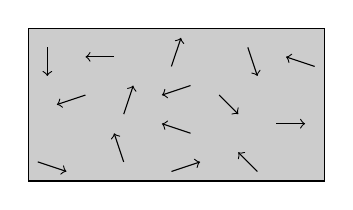
\begin{tikzpicture}
\filldraw[fill = black!20!white, draw = black] (0,0) rectangle (.31\textwidth,.16\textwidth);
\draw[->] (.15\textwidth,.01\textwidth) -- (.18\textwidth,.02\textwidth);
\draw[->] (.23\textwidth,.14\textwidth) -- (.24\textwidth,.11\textwidth);
\draw[->] (.01\textwidth,.02\textwidth) -- (.04\textwidth,.01\textwidth);
\draw[->] (.02\textwidth,.14\textwidth) -- (.02\textwidth,.11\textwidth);
\draw[->] (.17\textwidth,.10\textwidth) -- (.14\textwidth,.09\textwidth);
\draw[->] (.10\textwidth,.07\textwidth) -- (.11\textwidth,.10\textwidth);
\draw[->] (.24\textwidth,.01\textwidth) -- (.22\textwidth,.03\textwidth);
\draw[->] (.26\textwidth,.06\textwidth) -- (.29\textwidth,.06\textwidth);
\draw[->] (.20\textwidth,.09\textwidth) -- (.22\textwidth,.07\textwidth);
\draw[->] (.09\textwidth,.13\textwidth) -- (.06\textwidth,.13\textwidth);
\draw[->] (.06\textwidth,.09\textwidth) -- (.03\textwidth,.08\textwidth);
\draw[->] (.10\textwidth,.02\textwidth) -- (.09\textwidth,.05\textwidth);
\draw[->] (.15\textwidth,.12\textwidth) -- (.16\textwidth,.15\textwidth);
\draw[->] (.17\textwidth,.05\textwidth) -- (.14\textwidth,.06\textwidth);
\draw[->] (.30\textwidth,.12\textwidth) -- (.27\textwidth,.13\textwidth);
\end{tikzpicture}
}
\subfloat[][Ferromagnetici]{
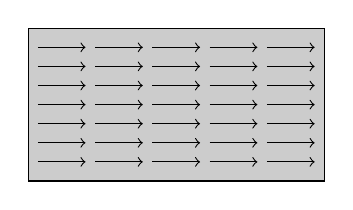
\begin{tikzpicture}
\filldraw[fill = black!20!white, draw = black] (0,0) rectangle (.31\textwidth,.16\textwidth);
\draw[->] (.01\textwidth,.02\textwidth) -- (.06\textwidth,.02\textwidth);
\draw[->] (.07\textwidth,.02\textwidth) -- (.12\textwidth,.02\textwidth);
\draw[->] (.13\textwidth,.02\textwidth) -- (.18\textwidth,.02\textwidth);
\draw[->] (.19\textwidth,.02\textwidth) -- (.24\textwidth,.02\textwidth);
\draw[->] (.25\textwidth,.02\textwidth) -- (.30\textwidth,.02\textwidth);

\draw[->] (.01\textwidth,.04\textwidth) -- (.06\textwidth,.04\textwidth);
\draw[->] (.07\textwidth,.04\textwidth) -- (.12\textwidth,.04\textwidth);
\draw[->] (.13\textwidth,.04\textwidth) -- (.18\textwidth,.04\textwidth);
\draw[->] (.19\textwidth,.04\textwidth) -- (.24\textwidth,.04\textwidth);
\draw[->] (.25\textwidth,.04\textwidth) -- (.30\textwidth,.04\textwidth);

\draw[->] (.01\textwidth,.06\textwidth) -- (.06\textwidth,.06\textwidth);
\draw[->] (.07\textwidth,.06\textwidth) -- (.12\textwidth,.06\textwidth);
\draw[->] (.13\textwidth,.06\textwidth) -- (.18\textwidth,.06\textwidth);
\draw[->] (.19\textwidth,.06\textwidth) -- (.24\textwidth,.06\textwidth);
\draw[->] (.25\textwidth,.06\textwidth) -- (.30\textwidth,.06\textwidth);

\draw[->] (.01\textwidth,.08\textwidth) -- (.06\textwidth,.08\textwidth);
\draw[->] (.07\textwidth,.08\textwidth) -- (.12\textwidth,.08\textwidth);
\draw[->] (.13\textwidth,.08\textwidth) -- (.18\textwidth,.08\textwidth);
\draw[->] (.19\textwidth,.08\textwidth) -- (.24\textwidth,.08\textwidth);
\draw[->] (.25\textwidth,.08\textwidth) -- (.30\textwidth,.08\textwidth);

\draw[->] (.01\textwidth,.10\textwidth) -- (.06\textwidth,.10\textwidth);
\draw[->] (.07\textwidth,.10\textwidth) -- (.12\textwidth,.10\textwidth);
\draw[->] (.13\textwidth,.10\textwidth) -- (.18\textwidth,.10\textwidth);
\draw[->] (.19\textwidth,.10\textwidth) -- (.24\textwidth,.10\textwidth);
\draw[->] (.25\textwidth,.10\textwidth) -- (.30\textwidth,.10\textwidth);

\draw[->] (.01\textwidth,.12\textwidth) -- (.06\textwidth,.12\textwidth);
\draw[->] (.07\textwidth,.12\textwidth) -- (.12\textwidth,.12\textwidth);
\draw[->] (.13\textwidth,.12\textwidth) -- (.18\textwidth,.12\textwidth);
\draw[->] (.19\textwidth,.12\textwidth) -- (.24\textwidth,.12\textwidth);
\draw[->] (.25\textwidth,.12\textwidth) -- (.30\textwidth,.12\textwidth);

\draw[->] (.01\textwidth,.14\textwidth) -- (.06\textwidth,.14\textwidth);
\draw[->] (.07\textwidth,.14\textwidth) -- (.12\textwidth,.14\textwidth);
\draw[->] (.13\textwidth,.14\textwidth) -- (.18\textwidth,.14\textwidth);
\draw[->] (.19\textwidth,.14\textwidth) -- (.24\textwidth,.14\textwidth);
\draw[->] (.25\textwidth,.14\textwidth) -- (.30\textwidth,.14\textwidth);
\end{tikzpicture}
}\\
\subfloat[][Antiferromagnetici]{
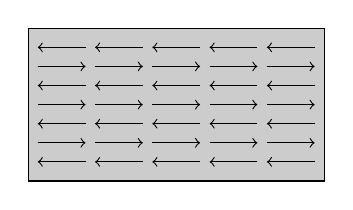
\begin{tikzpicture}
\filldraw[fill = black!20!white, draw = black] (0,0) rectangle (.31\textwidth,.16\textwidth);

\draw[->] (.06\textwidth,.02\textwidth) -- (.01\textwidth,.02\textwidth);
\draw[->] (.12\textwidth,.02\textwidth) -- (.07\textwidth,.02\textwidth);
\draw[->] (.18\textwidth,.02\textwidth) -- (.13\textwidth,.02\textwidth);
\draw[->] (.24\textwidth,.02\textwidth) -- (.19\textwidth,.02\textwidth);
\draw[->] (.30\textwidth,.02\textwidth) -- (.25\textwidth,.02\textwidth);

\draw[->] (.01\textwidth,.04\textwidth) -- (.06\textwidth,.04\textwidth);
\draw[->] (.07\textwidth,.04\textwidth) -- (.12\textwidth,.04\textwidth);
\draw[->] (.13\textwidth,.04\textwidth) -- (.18\textwidth,.04\textwidth);
\draw[->] (.19\textwidth,.04\textwidth) -- (.24\textwidth,.04\textwidth);
\draw[->] (.25\textwidth,.04\textwidth) -- (.30\textwidth,.04\textwidth);

\draw[->] (.06\textwidth,.06\textwidth) -- (.01\textwidth,.06\textwidth);
\draw[->] (.12\textwidth,.06\textwidth) -- (.07\textwidth,.06\textwidth);
\draw[->] (.18\textwidth,.06\textwidth) -- (.13\textwidth,.06\textwidth);
\draw[->] (.24\textwidth,.06\textwidth) -- (.19\textwidth,.06\textwidth);
\draw[->] (.30\textwidth,.06\textwidth) -- (.25\textwidth,.06\textwidth);

\draw[->] (.01\textwidth,.08\textwidth) -- (.06\textwidth,.08\textwidth);
\draw[->] (.07\textwidth,.08\textwidth) -- (.12\textwidth,.08\textwidth);
\draw[->] (.13\textwidth,.08\textwidth) -- (.18\textwidth,.08\textwidth);
\draw[->] (.19\textwidth,.08\textwidth) -- (.24\textwidth,.08\textwidth);
\draw[->] (.25\textwidth,.08\textwidth) -- (.30\textwidth,.08\textwidth);

\draw[->] (.06\textwidth,.10\textwidth) -- (.01\textwidth,.10\textwidth);
\draw[->] (.12\textwidth,.10\textwidth) -- (.07\textwidth,.10\textwidth);
\draw[->] (.18\textwidth,.10\textwidth) -- (.13\textwidth,.10\textwidth);
\draw[->] (.24\textwidth,.10\textwidth) -- (.19\textwidth,.10\textwidth);
\draw[->] (.30\textwidth,.10\textwidth) -- (.25\textwidth,.10\textwidth);

\draw[->] (.01\textwidth,.12\textwidth) -- (.06\textwidth,.12\textwidth);
\draw[->] (.07\textwidth,.12\textwidth) -- (.12\textwidth,.12\textwidth);
\draw[->] (.13\textwidth,.12\textwidth) -- (.18\textwidth,.12\textwidth);
\draw[->] (.19\textwidth,.12\textwidth) -- (.24\textwidth,.12\textwidth);
\draw[->] (.25\textwidth,.12\textwidth) -- (.30\textwidth,.12\textwidth);

\draw[->] (.06\textwidth,.14\textwidth) -- (.01\textwidth,.14\textwidth);
\draw[->] (.12\textwidth,.14\textwidth) -- (.07\textwidth,.14\textwidth);
\draw[->] (.18\textwidth,.14\textwidth) -- (.13\textwidth,.14\textwidth);
\draw[->] (.24\textwidth,.14\textwidth) -- (.19\textwidth,.14\textwidth);
\draw[->] (.30\textwidth,.14\textwidth) -- (.25\textwidth,.14\textwidth);
\end{tikzpicture}
}
\subfloat[][Ferrimagnetici]{
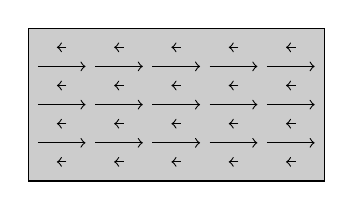
\begin{tikzpicture}
\filldraw[fill = black!20!white, draw = black] (0,0) rectangle (.31\textwidth,.16\textwidth);
\draw[->] (.04\textwidth,.02\textwidth) -- (.03\textwidth,.02\textwidth);
\draw[->] (.10\textwidth,.02\textwidth) -- (.09\textwidth,.02\textwidth);
\draw[->] (.16\textwidth,.02\textwidth) -- (.15\textwidth,.02\textwidth);
\draw[->] (.22\textwidth,.02\textwidth) -- (.21\textwidth,.02\textwidth);
\draw[->] (.28\textwidth,.02\textwidth) -- (.27\textwidth,.02\textwidth);

\draw[->] (.01\textwidth,.04\textwidth) -- (.06\textwidth,.04\textwidth);
\draw[->] (.07\textwidth,.04\textwidth) -- (.12\textwidth,.04\textwidth);
\draw[->] (.13\textwidth,.04\textwidth) -- (.18\textwidth,.04\textwidth);
\draw[->] (.19\textwidth,.04\textwidth) -- (.24\textwidth,.04\textwidth);
\draw[->] (.25\textwidth,.04\textwidth) -- (.30\textwidth,.04\textwidth);

\draw[->] (.04\textwidth,.06\textwidth) -- (.03\textwidth,.06\textwidth);
\draw[->] (.10\textwidth,.06\textwidth) -- (.09\textwidth,.06\textwidth);
\draw[->] (.16\textwidth,.06\textwidth) -- (.15\textwidth,.06\textwidth);
\draw[->] (.22\textwidth,.06\textwidth) -- (.21\textwidth,.06\textwidth);
\draw[->] (.28\textwidth,.06\textwidth) -- (.27\textwidth,.06\textwidth);

\draw[->] (.01\textwidth,.08\textwidth) -- (.06\textwidth,.08\textwidth);
\draw[->] (.07\textwidth,.08\textwidth) -- (.12\textwidth,.08\textwidth);
\draw[->] (.13\textwidth,.08\textwidth) -- (.18\textwidth,.08\textwidth);
\draw[->] (.19\textwidth,.08\textwidth) -- (.24\textwidth,.08\textwidth);
\draw[->] (.25\textwidth,.08\textwidth) -- (.30\textwidth,.08\textwidth);

\draw[->] (.04\textwidth,.10\textwidth) -- (.03\textwidth,.10\textwidth);
\draw[->] (.10\textwidth,.10\textwidth) -- (.09\textwidth,.10\textwidth);
\draw[->] (.16\textwidth,.10\textwidth) -- (.15\textwidth,.10\textwidth);
\draw[->] (.22\textwidth,.10\textwidth) -- (.21\textwidth,.10\textwidth);
\draw[->] (.28\textwidth,.10\textwidth) -- (.27\textwidth,.10\textwidth);

\draw[->] (.01\textwidth,.12\textwidth) -- (.06\textwidth,.12\textwidth);
\draw[->] (.07\textwidth,.12\textwidth) -- (.12\textwidth,.12\textwidth);
\draw[->] (.13\textwidth,.12\textwidth) -- (.18\textwidth,.12\textwidth);
\draw[->] (.19\textwidth,.12\textwidth) -- (.24\textwidth,.12\textwidth);
\draw[->] (.25\textwidth,.12\textwidth) -- (.30\textwidth,.12\textwidth);

\draw[->] (.04\textwidth,.14\textwidth) -- (.03\textwidth,.14\textwidth);
\draw[->] (.10\textwidth,.14\textwidth) -- (.09\textwidth,.14\textwidth);
\draw[->] (.16\textwidth,.14\textwidth) -- (.15\textwidth,.14\textwidth);
\draw[->] (.22\textwidth,.14\textwidth) -- (.21\textwidth,.14\textwidth);
\draw[->] (.28\textwidth,.14\textwidth) -- (.27\textwidth,.14\textwidth);
\end{tikzpicture}
}
\end{figure}

Per materiali  diamagnetici e paramagnetici isotropi la magnetizzazione è in genere parallela e proporzionale ad $\T{h}$:
\begin{equation}
\label{eq:2magnetiz1}
\T{m} = \chi \T{h}
\end{equation}
\begin{equation}
\label{eq:2magnetiz2}
\T{b}= \mu_0 \left(1+\chi\right)\T{h} = \mu \T{h} .
\end{equation}

La costante di proporzionalità $\chi$ è detta \textit{suscettività elettrica}, dipende dalla temperatura ed è negativa per i diamagnetici e positiva per i paramagnetici; nella maggior parte dei casi è dell'ordine di $10^{-4}-10^{-5}$.

Nel caso di anisotropie nei materiali  $\chi$ e $\mu$  in Eq. \eqref{eq:2magnetiz2} diventano tensori del secondo ordine:
 \begin{equation}
\label{eq:2magnetiz3}
\T{m} = \TT{\chi} \T{h}
\end{equation}
\begin{equation}
\label{eq:2magnetiz4}
\T{b}= \mu_0 \left(\TT{I}+\TT{\chi}\right)\T{h} = \TT{\mu} \T{h} .
\end{equation}


Per la caratterizzazione della legge costitutiva nei materiali ferromagnetici è necessaria l'analisi della loro  natura isteretica. In fig. \ref{fig:2.4} è mostrato un tipico grafico $\T{h}~-~\T{b}$ per un materiale a comportamento isteretico.

\begin{figure}[htp]
\centering
\caption{Curva di isteresi magnetica}
\label{fig:2.5}
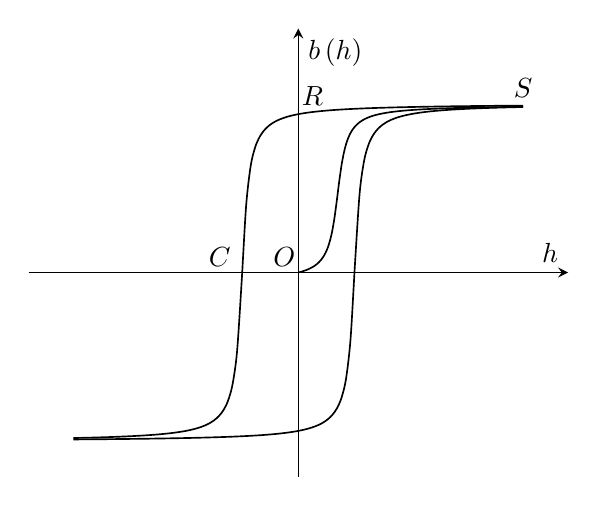
\begin{tikzpicture}
\begin{axis}[ylabel = $\T{b}\left(\T{h}\right)$,
			 xlabel = $\T{h}$,
			 ticks = none, 
			 ymax = 1100,
			 axis x line = middle, 
			 axis y line = middle, 
			 enlargelimits,
			 semithick]
\addplot[samples = 100, smooth, domain=-40:40]
{10*atan(x-10)};
\addplot[samples = 100, smooth, domain=-40:40]
{10*atan(x+10)};
\addplot[samples = 100, smooth, domain=0:40]
{(5*atan(0.8*(x-7))-5*atan(-0.8*7))*10*atan(30)/(5*atan(0.8*30)-5*atan(-0.8*7))};
\draw (-2.5,80) node {$O$}; %label
\draw (40,980) node {$S$}; %label
\draw (2.5,940) node {$R$}; %label
\draw (-14,80) node {$C$}; %label
\end{axis}
\end{tikzpicture}
\end{figure}

Nel punto $O$ nessun campo magnetico $\T{h}$ è applicato e i momenti di dipolo all'interno dei domini hanno direzioni randomatiche ($\T{m} = 0$).  
Con l'applicazione di un campo magnetico esterno i domini tendono ad allinearvisi e il materiale si muove lungo la curva $O-S$ in cui l'induzione magnetica cresce con $\T{h}$. 

Nel punto $S$ il materiale è saturo e i tutti i domini sono allineati al campo applicato. Diminuendo $\T{h}$ il campo si muove lungo la linea $S-R$, poiché il campo generato dai  domini contribuisce a mantenerne l'allineamento. 

Nel punto $R$ il materiale è nella condizione operativa e possiede un'\textit{induzione residua} $\T{b_r}$. 
Per poter tornare ad induzione magnetica nulla è necessario applicare un campo di verso opposto, muovendosi fino al punto $C$, la cui ascissa è detta \textit{coercitività} ($\T{h_c}$).  Il materiale è quindi vincolato a muoversi lungo l'anello isteretico e non può tornare alla curva $O-S$.

I materiali ferromagnetici si classificano, a seconda delle loro caratteristiche di coercitività e permeabilità, in:
\begin{description}
\item[Materiali soffici] Questi materiali hanno alta permeabilità e bassa coercitività ($\T{h_c}<10^3 \frac{\text{A}}{\text{m}}$) e sono quindi facili da magnetizzare e smagnetizzare. 

Vengono pertanto usati come canali per condurre o amplificare il flusso magnetico in trasformatori, motori, elettromagneti, induttori, ecc.
\item[Materiali duri] Al contrario, questi materiali hanno permeabilità relativamente bassa, alta coercitività ($\T{h_c}>10^4 \frac{\text{A}}{\text{m}}$)e sono difficili da magnetizzare e smagnetizzare. Sono utilizzati pertanto come magneti permanenti.
\end{description}

\begin{figure}[htb]
\centering
\caption{Curva di isteresi: confronto fra materiali morbidi (linea continua) e duri (linea tratteggiata)}
\label{fig:2.6}
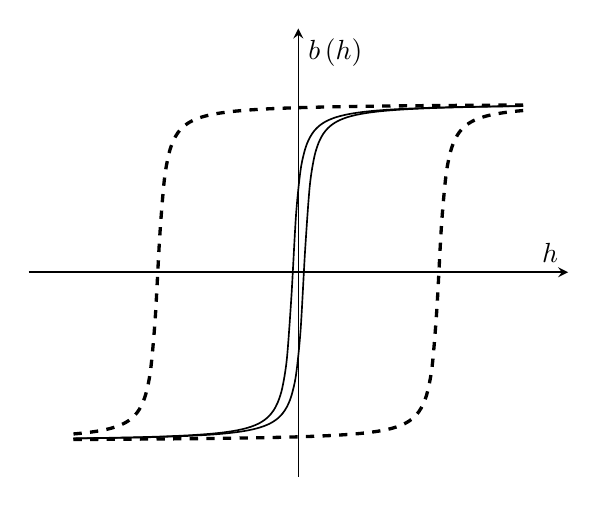
\begin{tikzpicture}
\begin{axis}[ylabel = $\T{b}\left(\T{h}\right)$,
			 xlabel = $\T{h}$,
			 ticks = none, 
			 ymax = 1100,
			 axis x line = middle, 
			 axis y line = middle, 
			 enlargelimits,
			 semithick]
\addplot[samples = 100, smooth, domain=-40:40]
{10*atan(x-1)};
\addplot[samples = 100, smooth, domain=-40:40]
{10*atan(x+1)};
\addplot[samples = 100, smooth, domain=-40:40, dashed, very thick]
{10*atan(x-25)};
\addplot[samples = 100, smooth, domain=-40:40, dashed, very thick]
{10*atan(x+25)};
\end{axis}
\end{tikzpicture}
\end{figure}

La tipica condizione operativa per i magneti morbidi è quella della ripida retta tra i due punti di saturazione inferiore e superiore. La linearità di questo tratto  e il valore estremamente basso di coercitività giustificano l'utilizzo delle relazioni \eqref{eq:2magnetiz1} e \eqref{eq:2magnetiz2} anche nel caso di materiali ferromagnetici, purché il campo applicato non sia eccessivo ($\T{b}< 1 \text{T}$, \citep{bossavit_computational_1998}). 
In questo caso $\chi$ varia tra $10^{3}$ e $10^{5}$.

Portando al limite le caratteristiche dei materiali magnetici soffici, si definisce il conduttore magnetico perfetto (\textit{perfect magnetic conductor, PMC}) come il materiale avente le seguenti proprietà:
\begin{equation}
\label{eq:2pmc}
\mu \rightarrow \infty,\qquad \T{h}\rightarrow 0.
\end{equation}

I magneti permanenti, magnetizzati durante il processo di produzione, hanno come condizione di riposo il punto $R$ di Figura \ref{fig:2.5} e in condizioni operative restano nell'intorno di questo punto (tratto lineare). Per questa classe di materiali è pertanto giustificato utilizzare il seguente modello:
\begin{align}
\label{eq:2costmag}
\T{m(h)}&=\TT{\chi}\T{h}+\T{m_r}\nonumber \\
\T{b(h)}&=\mu_0(\T{h}+\left(\TT{\chi}\T{h}+\T{m_r}\right) \nonumber\\
&=\mu_0\left(\TT{I}+\TT{\chi}\right)\T{h}+\mu_0 \T{m_r} \nonumber \\
&=\TT{\mu}\T{h}+\mu_0 \T{m_r}\nonumber\\
&= \TT{\mu}\T{h}+\T{b_r}.
\end{align}
\section{Regimi speciali}
Non sempre è necessario applicare il modello completo fornito dalle equazioni di Maxwell per la risoluzione di problemi di natura elettromagnetica. In molte applicazioni, infatti, la dinamica dei campi è parzialmente o interamente trascurabile perché più veloce della variazione delle condizioni al contorno associate. 

Vengono qui brevemente introdotti due modelli, adottati per le successive analisi.

\subsection{Regime quasi-stazionario magnetico}
A basse frequenze e se le dimensioni caratteristiche del problema sono molto inferiori alle lunghezze d'onda proprie del campo elettromagnetico si può applicare l'approssimazione quasi-stazionaria: in queste condizioni il campo elettromagnetico varia con tempi più lunghi di quelli necessari alla sua propagazione e si può pertanto assumere che la velocità di quest'ultima sia infinita (qualsiasi variazione nel campo elettromagnetico è percepita istantaneamente in tutto il dominio). I tre modelli quasi-stazionari più utilizzati sono \citep{larsson_electromagnetics_2007}:
\begin{itemize}
\item Modello quasi-stazionario magnetico (\textit{MQS})
\item Modello quasi-stazionario elettrico (\textit{EQS})
\item Modello di Darwin
\end{itemize}

Viene posta attenzione qui solo al regime \textit{MQS}, utilizzato nelle simulazioni successive.

Nel regime quasi-stazionario magnetico si presuppone che la variazione del campo $\partial_t \T{d}$ dia un contributo trascurabile rispetto alla corrente libera $\T{j}$; tale termine viene pertanto eliminato nell'equazione \eqref{eq:2max3}. Questo porta alla riscrittura delle equazioni \eqref{eq:2max1}-\eqref{eq:2max4}:
\begin{equation}
	\label{eq:2max1qs}
	\rot\left(\T{e}\right)=-\partial_t \T{b},
\end{equation}
\begin{equation}
	\label{eq:2max2qs}
	\dive\left(\T{d}\right)=\rho,
\end{equation}
\begin{equation}
	\label{eq:2max3qs}
	\rot\left(\T{h}\right)=\T{j},
\end{equation}
\begin{equation}
	\label{eq:2max4qs}
	\dive\left(\T{b}\right)=0,
\end{equation}
con
\begin{equation}
\label{eq:2corr1qs}
\dive\left(\T{j}\right) = 0.
\end{equation}

Dalla prima equazione si evince che il campo magnetico e la  sua induzione seguono staticamente la variazione temporale di corrente $\T{j}$ e non dipendono dalla controparte elettrica\footnote{In realtà i due campi continuano ad interagire laddove la corrente $\T{j}$ dipende dal campo elettrico. Particolare attenzione va posta, pertanto, nella corretta modellazione del comportamento delle regioni metalliche (Capitolo \ref{cap:boundary}).}. 
Il campo elettrico è invece influenzato separatamente nelle sue parti di rotore e divergenza dalle equazioni \eqref{eq:2max1qs} e \eqref{eq:2max2qs}.
Questa separazione suggerisce una scomposizione del campo $\T{e}$ in due parti:
\begin{equation}
\label{eq:2scomp_e}
\T{e} = \T{e_c}+\T{e_f},
\end{equation} 
dove $\T{e_c}$ è irrotazionale ed è identificato tramite la sola legge di Coulomb:
\begin{equation}
\label{eq:2e_coulomb}
\left\{
\begin{array}{l}
\dive\left(\TT{\varepsilon} \T{e_c}\right) = \rho\\
\rot\left(\T{e_c}\right) = 0
\end{array}
\right.
\end{equation}
e $\T{e_f}$ è solenoidale e segue la legge di Faraday:
\begin{equation}
\label{eq:2e_faraday}
\left\{
\begin{array}{l}
\dive\left(\TT{\varepsilon} \T{e_f}\right) = 0\\
\rot\left(\T{e_f}\right) =\partial_t \T{b}.
\end{array}
\right.
\end{equation}

Questa separazione suggerisce la seguente strategia di calcolo:
\begin{enumerate}
\item Risoluzione delle equazioni \eqref{eq:2max3qs} e \eqref{eq:2max4qs} per ottenere staticamente la storia temporale di $\T{b}$ e $\T{h}$ ;
\item Risoluzione della prima delle equazioni \eqref{eq:2e_coulomb} per la determinazione della parte irrotazionale di $\T{e}$ ($\T{e_c}$);
\item Determinazione della storia temporale di $\T{e_f}$ mediante la seconda delle \eqref{eq:2e_faraday}.
\end{enumerate}


\subsection{Regime stazionario}
In assenza completa di variazioni temporali si può ritenere nullo qualsiasi contributo dinamico. In questo caso anche il termine $\partial_t\T{b}$ è nullo e le equazioni sono pienamente disaccoppiate, permettendo lo studio separato di elettrostatica e magnetostatica.
\begin{equation}
\label{eq:2max12s}
\left\{
\begin{aligned}
\rot\left(\T{e}\right)=0\\
\dive\left(\T{d}\right)=\rho
\end{aligned}
\right.
\end{equation}
e
\begin{equation}
\label{eq:2max34s}
\left\{
\begin{aligned}
\rot\left(\T{h}\right)=\T{j}\\
\dive\left(\T{b}\right)=0.
\end{aligned}
\right.
\end{equation}
\subsection{Condizioni di applicabilità}
Dopo aver introdotto i diversi regimi ci chiediamo quali condizioni devono essere verificate perché la loro applicazione sia giustificata.
Un primo criterio di applicazione dei regimi quasi-stazionari \citep{zaglmayr_high_2006} è il confronto tra i tempi di propagazione delle onde elettromagnetiche all'interno del dominio di analisi e i tempi caratteristici di variazione delle sorgenti dei campi (cariche e correnti). In regime armonico si ha:
\begin{equation}
\label{eq:2regimi1}
\tau_{\lambda} = \frac{L}{c} \gg \frac{2\pi}{\omega_s} = \tau_s,
\end{equation}
dove $L$ è la dimensione caratteristica del dominio, $c$ è la velocità di propagazione delle onde e $\omega_s$ è la pulsazione caratteristica delle sorgenti di campo.\\

Si può tuttavia analizzare più approfonditamente l'ordine di grandezza delle quantità che possono venire trascurate nella scelta dei diversi regimi \citep{emson_methods_1988}; in quest'ottica approssimiamo le derivate spaziali e temporali utilizzando la lunghezza caratteristica $L$ e un tempo caratteristico $\tau$. 

Iniziamo cercando un criterio per discernere i campi di applicabilità dei regimi \textit{MQS} e dinamico. Chiamiamo $\hat{h}$ il campo che soddisfa l'Eq. \eqref{eq:2max3qs}:
\begin{equation}
\label{eq:2regimi2}
\hat{h} L = j L^2 \longrightarrow \hat{h} =  j L
\end{equation}   
e $h$ il campo che soddisfa l'Eq. \eqref{eq:2max3}:
\begin{equation}
\label{eq:2regimi3}
h =  j L +  \varepsilon \frac{e}{\tau} L.
\end{equation}

L'errore tra $\hat{h}$ e $h$ è dato da
\begin{equation}
\label{eq:2regimi4}
\Delta h =  \varepsilon \frac{e}{\tau},
\end{equation}
dove
\begin{equation}
\label{eq:2regimi5}
e L = \mu \frac{\hat{h}}{\tau} L^2 \longrightarrow e = \mu \frac{\hat{h}}{\tau} L.
\end{equation}

Si noti che è stato utilizzato $\hat{h}$ in Eq. \eqref{eq:2regimi5} e non $h$. Si ottiene così una stima dell'errore:
\begin{align}
\label{eq:2regime6_a}
\Delta h = \mu \varepsilon j \frac{L^3}{\tau^2}, \\
\label{eq:2regime6_b}
\frac{\Delta h}{\hat{h}} = \mu \varepsilon \frac{L^2}{\tau^2}.
\end{align}

Se $\Delta h$ è trascurabile rispetto a $\hat{h}$ è ragionevole l'utilizzo dell'approccio \textit{MQS}.\\

Cerchiamo ora una stima dell'intensità di campo elettrico indotta dalla variazione di induzione magnetica, utile per avere un criterio di scelta fra regime \textit{MQS} e regime stazionario:
\begin{align}
\label{eq:2regimi7_a}
hL= jL^2 \longrightarrow \frac{h}{L} &= j\\
\label{eq:2regimi7_b}
eL= \frac{b}{\tau} L^2 \longrightarrow\frac{e}{L} &= \frac{\mu h}{\tau},
\end{align} 
da cui
\begin{equation}
\label{eq:2regimi8}
e = \frac{\mu j L^2}{\tau}.
\end{equation}

Se tale valore è piccolo il modello stazionario è applicabile con buona approssimazione.\\

Per dimostrare l'applicabilità del regime MQS ed avere una stima dell'errore commesso, il criterio sopra mostrato è stato verificato per dimensioni e tempi conservativi rispetto a quelli tipici per gli attuatori del sistema di controllo:
\begin{equation}
\nonumber
\begin{array}{l}
L = 0.1 \text{m},\\
\tau = 10^-5 \text{s}.
\end{array}
\end{equation}
Si ottiene:
\begin{equation}
\nonumber
\begin{array}{l}
\frac{\Delta h}{\hat{h}} = 10^{-6},\\
e = 10^{-3}j.
\end{array}
\end{equation}
Guardando il primo dei due termini si può ritenere appropriato l'utilizzo del regime quasi-stazionario in sostituzione al regime dinamico completo. Tuttavia l'ordine di grandezza del campo elettrico non permette di stabilire a priori l'applicabilità del regime stazionario completo.

\section{Potenziale scalare e potenziale vettore}
\label{subsec:1potenziale}
\subsection{Regime dinamico}
Scegliamo ora una formulazione che permetta di soddisfare a priori la solenoidalità del campo $\T{b}$ (Eq. \eqref{eq:2max4}). Introduciamo quindi il \textit{potenziale vettore} $\T{a}$ tale per cui
\begin{equation}
\label{eq:2potvet}
\rot\left(\T{a}\right) = \T{b}.
\end{equation}

Sostituendo nell'equazione \eqref{eq:2max1} l'induzione magnetica secondo la relazione di cui sopra, si ottiene:
\begin{align}
\label{eq:2potvet2}
\rot\left(\T{e}\right)=-\partial_t \rot\left(\T{a}\right)\nonumber\\
\rot\left(\T{e}\right)=- \rot\left(\partial_t\T{a}\right)\nonumber\\
\rot\left(\T{e}+\partial_t\T{a}\right)=0.
\end{align}


Poiché la quantità $\T{e}+\partial_t\T{a}$ è irrotazionale è possibile introdurre un secondo potenziale, questa volta \textit{scalare}, $\phi$:
\begin{equation}
\label{eq:2potsca}
\T{e}+\partial_t\T{a} = - \grad\left(\phi\right)
\end{equation}
da cui
\begin{equation}
\label{eq:2potsca2}
\T{e} = - \grad\left(\phi\right)-\partial_t\T{a}
\end{equation}

Possiamo quindi ora riscrivere le Eq. \eqref{eq:2max2} e \eqref{eq:2max3}, utilizzando i potenziali appena definiti, utilizzando le leggi costitutive \eqref{eq:2costel} e \eqref{eq:2costmag}:
\begin{align}
\label{eq:2pot1}
\dive\left(\T{d}\right)&=\rho\nonumber\\
\dive\left(\TT{\varepsilon}\T{e}\right) &= \rho \nonumber\\
\dive \left[ \TT{\varepsilon} \cdot \grad \left( \phi \right) \right] + \dive \left[ \TT{\varepsilon} \partial_t \left( \T{a} \right) \right] &= -\rho \nonumber\\
\dive \left( \TT{\varepsilon} \right) \cdot \grad \left( \phi \right) + \TT{\varepsilon} : \grad \left[ \grad \left( \phi \right) \right] + & \nonumber\\
+\dive \left( \TT{\varepsilon} \right) \cdot \partial_t \left( \T{a} \right) + \TT{\varepsilon} : \grad \left[ \partial_t \left( \T{a} \right) \right] & = - \rho\nonumber\\
\dive \left( \TT{\varepsilon} \right) \cdot \left[ \grad \left( \phi \right) +\partial_t \left( \T{a} \right) \right]+&\nonumber\\
+\TT{\varepsilon} :  \grad \left[ \grad \left( \phi \right)  + \partial_t \left( \T{a} \right) \right]& = - \rho
\end{align}
e
\begin{align}
\label{eq:2pot2}
\rot \left( \T{h} \right) =& \T{j}+ \partial_t \T{d} \nonumber\\
\rot \left[ \TT{\mu}^{-1} \left( \T{b}-\T{b_r} \right) \right] =& \T{j}+\partial_t \left(\TT{\varepsilon} \T{e} \right)\nonumber\\
\rot \left[ \TT{\mu}^{-1} \rot\left(\T{a}\right) \right] =& \T{j}+\rot\left(\TT{\mu}^{-1}\T{b_r}\right)-\partial_t \left[\TT{\varepsilon} \left(\partial_t \T{a}+\grad\left(\phi\right)\right) \right].
\end{align}

Si riscrivano ora (con perdita di generalità) le equazioni \eqref{eq:2pot1} e \eqref{eq:2pot2} nel caso in cui in ciascun dominio del problema le permeabilità elettrica e magnetica siano costanti e allineate con le rispettive intensità di campo ed esprimibili quindi tramite gli scalari $\varepsilon$ e $\mu$.
Si ha allora:
\begin{align}
\label{eq:2pot1bis}
\lap\left(\phi\right)+\dive\left( \partial_t \T{a} \right) = -\varepsilon^{-1}\rho
\end{align}
e\footnote{Viene qui utilizzata l'identità vettoriale +$\rot\left[\rot\left(\T{a}\right)\right]=\grad\left[\dive\left(\T{a}\right)\right]-\lap\left(\T{a}\right)$}
\begin{align}
\label{eq:2pot2bis}
\rot \left[\rot\left(\T{a}\right) \right] =& \mu\T{j}+\rot\left(\T{b_r}\right)-\mu\TT{\varepsilon}\left[\partial_{tt}\T{a}+\partial_t \grad\left(\phi\right)\right]\nonumber\\
\grad\left[\dive\left(\T{a}\right)\right]-\lap\left(\T{a}\right) =& \mu\T{j}+\rot\left(\T{b_r}\right)+\nonumber\\
&-\mu\TT{\varepsilon}\left[\partial_{tt}\T{a}+\partial_t \grad\left(\phi\right)\right].
\end{align}

Le equazioni \eqref{eq:2pot1bis} e \eqref{eq:2pot2bis} possono sembrare adeguate per la risoluzione del problema nelle due variabili $\T{a}$ e ${\phi}$. Tuttavia per la caratterizzazione completa del potenziale vettore non è sufficiente la definizione del suo rotore ma occorre anche quella del suo gradiente \citep{griffiths_introduction_2013}. Tale condizione è chiamata \textit{condizione di gabbia} (gauge condition). Tra le varie possibilità la più utilizzata per il modello dinamico completo è la condizione di Lorentz:
\begin{equation}
\label{eq:2lorentzgauge}
\dive\left(\T{a}\right) = -\mu\TT{\varepsilon}\partial_{t} \phi.
\end{equation}

Sostituendo l'equazione \eqref{eq:2lorentzgauge} nelle \eqref{eq:2pot1} e \eqref{eq:2pot2} otteniamo
\begin{equation}
\label{eq:2pot3}
\lap\left({\phi}\right)-\mu\varepsilon\partial_{tt}\phi = -\varepsilon^{-1} \rho
\end{equation}
e
\begin{equation}
\label{eq:2pot4}
\mu\varepsilon\partial_{tt}\T{a}-\lap\left(\T{a}\right) = \mu\T{j}+\rot\left(\T{b_r}\right).
\end{equation}
\subsection{Regime quasi-stazionario}
Applicando la definizione del potenziale vettoriale alle Eq. \eqref{eq:2max1qs}-\eqref{eq:2max4qs} e ripercorrendo i passaggi appena svolti per le equazioni complete si ha:
\begin{align}
\label{eq:2pot1qs}
\varepsilon\left[ \lap\left(\phi\right)+\partial_t\left( \dive\left(\T{a}\right)\right)\right] = \rho,\\
\rot \left[\rot\left(\T{a}\right) \right] = \mu\T{j}+\rot\left(\T{b_r}\right).
\end{align}

In questo caso come condizione di gabbia scegliamo la più semplice condizione di Gauss:
\begin{equation}
\label{eq:2gaussgauge}
\dive\left(\T{a}\right) = 0,
\end{equation}
che porta anche in questo caso al disaccoppiamento delle equazioni:
\begin{equation}
\label{eq:2pot2qs}
\lap\left({\phi}\right) = \varepsilon^{-1} \rho
\end{equation}
e
\begin{equation}
\label{eq:2pot3qs}
-\lap\left(\T{a}\right) = \mu\T{j}+\rot\left(\T{b_r}\right)
\end{equation}
con
\begin{equation}
\label{eq:2pot4qs}
\left\{
\begin{aligned}
\T{b}&=\rot \left(\T{a}\right)\\
\T{e_c} &= -\grad\left(\phi\right)\\
\T{e_f} &= -\partial_t \T{a}.
\end{aligned}
\right.
\end{equation}

\subsection{Regime stazionario}
Completiamo la trattazione analizzando anche il regime stazionario. In questo caso, dalle equazioni \eqref{eq:2max12s} si ricava una diversa definizione del potenziale scalare:
\begin{align}
\label{eq:2pot1s}
\rot\left(\T{e}\right)=0\nonumber\\
\T{e} = - \grad\left(\phi\right),
\end{align}
da cui le equazioni
\begin{align}
\label{eq:2pot2s}
\varepsilon \lap\left(\phi\right) = \rho,\\
\rot \left[\rot\left(\T{a}\right) \right] = \mu\T{j}+\rot\left(\T{b_r}\right).
\end{align}
Anche in questo caso applichiamo la condizione di gabbia di Gauss:
\begin{equation}
\label{eq:2gaussgauge2}
\dive\left(\T{a}\right) = 0,
\end{equation}
da cui:
\begin{equation}
\label{eq:2pot3qs2}
\lap\left({\phi}\right) = \varepsilon^{-1} \rho
\end{equation}
e
\begin{equation}
\label{eq:2pot4qs2}
-\lap\left(\T{a}\right) = \mu\T{j}+\rot\left(\T{b_r}\right).
\end{equation}